%\documentclass[draft,a4paper,twoside,fleqn,11pt]{ethdissertation}
\documentclass[publish]{ethdissertation}
\batchmode
%%%%%%%%%%%%%%%%%%%%%%%%%%%%%%%%%%%%%%%%%%%%%%%%%%%%%%%%
% Subfiles
\usepackage{subfiles}
%%%%%%%%%%%%%%%%%%%%%%%%%%%%%%%%%%%%%%%%%%%%%%%%%%%%%%%%
% Combine with clearpage
\usepackage{afterpage}

%%%%%%%%%%%%%%%%%%%%%%%%%%%%%%%%%%%%%%%%%%%%%%%%%%%%%%%%
% Side captions
\usepackage{sidecap}
\renewcommand{\sidecaptionsep}{2em}

%%%%%%%%%%%%%%%%%%%%%%%%%%%%%%%%%%%%%%%%%%%%%%%%%%%%%%%%
% Hyperlinks
\usepackage{hyperref}

%%%%%%%%%%%%%%%%%%%%%%%%%%%%%%%%%%%%%%%%%%%%%%%%%%%%%%%%
% Text Symbols (alpha, phi ...)
\usepackage{textgreek} %nice greek letters everywhere


%%%%%%%%%%%%%%%%%%%%%%%%%%%%%%%%%%%%%%%%%%%%%%%%%%%%%%%%
% Supporting INFO

\usepackage{longtable}
\usepackage{lscape}
\newcommand{\si}{Supporting Information}
\newlength{\oldtabcolsep}
\setlength{\oldtabcolsep}{\tabcolsep}
\usepackage{xfrac}
\usepackage{csquotes}
\usetikzlibrary{positioning}

%%%%%%%%%%%%%%%%%%%%%%%%%%%%%%%%%%%%%%%%%%%%%%%%%%%%%%%%
% Handling of the references - Reference lib
%\usepackage[backend=biber,
%			style=alphabetic,
%			sorting=ynt]{biblatex}



\usepackage[sort,super,comma,compress]{natbib}
\bibliographystyle{unsrt}

%\usepackage{natmove}
%\renewcommand{\bibname}{References}

%% % Call as \square{\cite{key}} to work with lars
%% \newcommand*{\square}[1]{%
%%   \begingroup
%%     \romannumeral-`\x % remove space at the beginning of \setcitestyle
%%     \setcitestyle{numbers}%
%%     [#1]%
%%   \endgroup   
%% }

%%%%%%%%%%%%%%%%%%%%%%%%%%%%%%%%%%%%%%%%%%%%%%%%%%%%%%%%
% Math
\usepackage{bigdelim}

%%%%%%%%%%%%%%%%%%%%%%%%%%%%%%%%%%%%%%%%%%%%%%%%%%%%%%%%
% Footnotes
\renewcommand{\thefootnote}{\fnsymbol{footnote}}

%%%%%%%%%%%%%%%%%%%%%%%%%%%%%%%%%%%%%%%%%%%%%%%%%%%%%%%%
% Tables
\usepackage{multirow}

%%%%%%%%%%%%%%%%%%%%%%%%%%%%%%%%%%%%%%%%%%%%%%%%%%%%%%%%
% Special Itemization 
\usepackage[inline]{enumitem}
\usepackage{xstring}

%%%%%%%%%%%%%%%%%%%%%%%%%%%%%%%%%%%%%%%%%%%%%%%%%%%%%%%%
% Hyphenations
\hyphenation{zustands-summe di-poles Cou-lomb ma-cro-sco-pic}

%%%%%%%%%%%%%%%%%%%%%%%%%%%%%%%%%%%%%%%%%%%%%%%%%%%%%%%%
% Personal Commands 
\newcommand*\mycommand[1]{\texttt{\emph{#1}}}
\newcommand{\nc}{\newcommand}

\nc{\captitital}[1]{\textit{#1}}

\nc{\ie}{\textit{i.e.}}
\nc{\via}{\textit{via}}
\nc{\eg}{\textit{e.g.}}
\nc{\vs}{\textit{vs.}}
\newcommand{\cf}{\textit{cf.}}
\nc{\suppmat}{}
\nc{\suppmatv}{}

%==============================================================================
%==============================================================================
% SPECIFIC TO CH 1
%==============================================================================
%==============================================================================

\nc{\nitro}{\textsc{Nitro}}
\nc{\quino}{\textsc{Quino}}

\nc{\vase}{\textsc{Vase}}
\nc{\oneopen}{\textsc{Oneopen}}
%
\nc{\twoopen}{\textsc{Twoopen}}
%\nc{\twoopencone}{\textsc{Twoopen-cis-o}}
%\nc{\twoopenctwo}{\textsc{Twoopen-cis-p}}
%\nc{\twoopencco}{\textsc{Twoopen-cis-o}}
%\nc{\twoopenccp}{\textsc{Twoopen-cis-p}}
%\nc{\twoopent}{\textsc{Twoopen-trans}}

\nc{\twoopencone}{\textsc{Twoopen}-{\em cis}-$o$}
\nc{\twoopenctwo}{\textsc{Twoopen}-{\em cis}-$p$}
\nc{\twoopencco}{\textsc{Twoopen}-{\em cis}-$o$}
\nc{\twoopenccp}{\textsc{Twoopen}-{\em cis}-$p$}
\nc{\twoopent}{\textsc{Twoopen}-{\em trans}}

% David's
%\nc{\ciso}{\textsc{cis-o}}
%\nc{\cisp}{\textsc{cis-p}}
%\nc{\trans}{\textsc{trans}}
%
% Phil's
\nc{\ciso}{{\em cis-o}}
\nc{\cisp}{{\em cis-p}}
\nc{\trans}{{\em trans}}
%
\nc{\threeopencone}{\textsc{Threeopen} (\via{} \ciso{})}
\nc{\threeopenctwo}{\textsc{Threeopen} (\via{} \cisp{})}
\nc{\threeopent}{\textsc{Threeopen} (\via{} \trans{})}
\nc{\threeopen}{\textsc{Threeopen}}
\nc{\threeopenave}{\textsc{Threeopen} (Ave)}
\nc{\kitecone}{\textsc{Kite} (\via{} \ciso{})}
\nc{\kitectwo}{\textsc{Kite} (\via{} \cisp{})}
\nc{\kitet}{\textsc{Kite} (\via{} \trans{})}
\nc{\kite}{\textsc{Kite}}
\nc{\kiteave}{\textsc{Kite} (Ave)}
\nc{\dih}[3]{\IfEq{#3}{bar}{$\phi_{\mathrm{#1}\overline{#2}}$}{$\phi_{\mathrm{#1}#2}$}}

\nc{\dihnobar}[2]{$\phi_{\mathrm{#1}#2}$}
\nc{\dihbar}[2]{$\phi_{\mathrm{#1}\overline{#2}}$}

% {N,Q}{V,C,T}{l,m,h}{Nsph}-{0,1,X}{0,1,X}{0,1,X}{0,1,X}
\nc{\simu}[5]{\textsc{#1#2#3-#4}\-\textsc{-#5}}
\nc{\simup}[4]{\textsc{#1#2#3}\-\textsc{-#4}}
\nc{\simum}[5]{#1\_\textsc{#2#3#4}\-\textsc{-#5}}

\nc{\refsimov}[4]{Movie \textsc{#1#2#3}\-\textsc{-#4}}
\nc{\refsimovm}[5]{Movie #1\_\textsc{#2#3#4}\-\textsc{-#5}}

%==============================================================================
%==============================================================================
% SPECIFIC TO CH 3
%==============================================================================
%==============================================================================

\nc{\KXK}{\textsc{KXK}}
\nc{\KEK}{\textsc{KEK}}
\nc{\KGK}{\textsc{KG$_{\mathrm E}$K}}

\nc{\XTP}{\textsc{XTP}}
\nc{\GTP}{\textsc{GTP}}
\nc{\BTP}{\textsc{BTP}}

\nc{\CNFA}{\textsc{C$_{\mathrm A}$}}
\nc{\CNFB}{\textsc{C$_{\mathrm B}$}}

\nc{\TI}{\textsc{TI}}
\nc{\HR}{\textsc{HR}}
\nc{\CB}{\textsc{CB}}

\nc{\FWD}{\textsc{FWD}}
\nc{\BWD}{\textsc{BWD}}
\nc{\MIX}{\textsc{MIX}}

\nc{\SIMP}{\textsc{SIMP}}
\nc{\MBAR}{\textsc{MBAR}}
\nc{\EXTI}{\textsc{EXTI}}
\nc{\CFIT}{\textsc{CFIT}}

\nc{\BIAS}{\textsc{BIAS}}

\nc{\REF}{\textsc{REF}}
\nc{\REP}{\textsc{REP}}

\nc{\AAD}{\textsc{AAD}}
\nc{\MAD}{\textsc{AAD}}
\nc{\EOM}{\textsc{EOM}}


%==============================================================================
%==============================================================================
% SPECIFIC TO CH 4
%==============================================================================
%==============================================================================

\nc{\xim}{\xi_-}
\nc{\xip}{\xi_+}
\nc{\ximt}{\xi^{\mathrm{CB}}_-}
\nc{\xipt}{\xi^{\mathrm{CB}}_+}
\nc{\xic}{\xi_*}
\nc{\xio}{\xi_o}
\nc{\xiclose}{\xi_m}

% PHIL
% -----
%
\nc{\DCNT}{\textsc{DCNT}}
\nc{\TRUS}{\textsc{TRUS}}
\nc{\REUS}{\textsc{REUS}}
\nc{\CBUS}{\textsc{CBUS}}
%
\nc{\DCAN}{\textsc{DCAN}} % Direct counting analysis
\nc{\PMAT}{\textsc{PMAT}}
\nc{\WHAM}{\textsc{WHAM}}
\nc{\VFEP}{\textsc{VFEP}}
\nc{\UINT}{\textsc{UINT}} % umbrella integration
\nc{\TINT}{\textsc{TINT}} % true integration = force integration
%


\definecolor{colli}{HTML}{783632}
\definecolor{colna}{HTML}{69BC4E}
\definecolor{colk}{HTML}{7B49CA}
\definecolor{colrb}{HTML}{BBAB4E}
\definecolor{colcs}{HTML}{D052AE}
\definecolor{colh2o}{HTML}{4D6433}
\definecolor{coldmso}{HTML}{D44442}
\definecolor{colch3oh}{HTML}{63B09D}
\definecolor{colchcl3}{HTML}{58366F}
\definecolor{col12c4}{HTML}{C77C3D}
\definecolor{col15c5}{HTML}{798FC9}
\definecolor{col18c6}{HTML}{CD8597}

%% \newcommand{\ws}[1]{\IfEq{#1}{10_H2O}{{\color{colh2o} H$_2$O}}{\IfEq{#1}{11_DMSO}{{\color{coldmso} DMSO}}{\IfEq{#1}{12_CHCL3}{{\color{colchcl3} CHCl$_3$}}{\IfEq{#1}{13_CH3OH}{{\color{colch3oh} CH$_3$OH}}{%
%% \IfEq{#1}{H2O}{{\color{colh2o} H$_2$O}}{\IfEq{#1}{DMSO}{{\color{coldmso} DMSO}}{\IfEq{#1}{CHCL3}{{\color{colchcl3} CHCl$_3$}}{\IfEq{#1}{CH3OH}{{\color{colch3oh} CH$_3$OH}}}}}}}}}}

%% \newcommand{\wc}[1]{\IfEq{#1}{01_12C4}{{\color{col12c4} 12C4}}{\IfEq{#1}{02_15C5}{{\color{col15c5} 15C5}}{\IfEq{#1}{03_18C6}{{\color{col18c6} 18C6}}{%
%% \IfEq{#1}{12C4}{{\color{col12c4} 12C4}}{\IfEq{#1}{15C5}{{\color{col15c5} 15C5}}{\IfEq{#1}{18C6}{{\color{col18c6} 18C6}}{%
%% }}}}}}}
%% \newcommand{\wi}[1]{\IfEq{#1}{01_LI+}{{\color{colli} Li$^+$}}{\IfEq{#1}{02_NA+}{{\color{colna} Na$^+$}}{\IfEq{#1}{03_K+}{{\color{colk} K$^+$}}{\IfEq{#1}{04_RB+}{{\color{colrb} Rb$^+$}}{\IfEq{#1}{05_CS+}{{\color{colcs} Cs$^+$}}{%
%% \IfEq{#1}{LI+}{{\color{colli} Li$^+$}}{\IfEq{#1}{NA+}{{\color{colna} Na$^+$}}{\IfEq{#1}{K+}{{\color{colk} K$^+$}}{\IfEq{#1}{RB+}{{\color{colrb} Rb$^+$}}{\IfEq{#1}{CS+}{{\color{colcs} Cs$^+$}}{}}}}}}}}}}}


\newcommand{\ws}[1]{\IfEq{#1}{10_H2O}{{ H$_2$O}}{\IfEq{#1}{11_DMSO}{{ DMSO}}{\IfEq{#1}{12_CHCL3}{{ CHCl$_3$}}{\IfEq{#1}{13_CH3OH}{{ CH$_3$OH}}{%
\IfEq{#1}{H2O}{{ H$_2$O}}{\IfEq{#1}{DMSO}{{ DMSO}}{\IfEq{#1}{CHCL3}{{ CHCl$_3$}}{\IfEq{#1}{CH3OH}{{ CH$_3$OH}}}}}}}}}}

\newcommand{\wc}[1]{\IfEq{#1}{01_12C4}{{12C4}}{\IfEq{#1}{02_15C5}{{15C5}}{\IfEq{#1}{03_18C6}{{18C6}}{%
\IfEq{#1}{12C4}{{12C4}}{\IfEq{#1}{15C5}{{15C5}}{\IfEq{#1}{18C6}{{18C6}}{%
}}}}}}}
\newcommand{\wi}[1]{\IfEq{#1}{01_LI+}{{Li$^+$}}{\IfEq{#1}{02_NA+}{{Na$^+$}}{\IfEq{#1}{03_K+}{{K$^+$}}{\IfEq{#1}{04_RB+}{{Rb$^+$}}{\IfEq{#1}{05_CS+}{{Cs$^+$}}{%
\IfEq{#1}{LI+}{{Li$^+$}}{\IfEq{#1}{NA+}{{Na$^+$}}{\IfEq{#1}{K+}{{K$^+$}}{\IfEq{#1}{RB+}{{Rb$^+$}}{\IfEq{#1}{CS+}{{Cs$^+$}}{}}}}}}}}}}}

% phil prefers Ref. with superscripts...
\nc{\squarit}[1]{#1}
% David's way with square brackets...
%\nc{\squarit}[1]{~\square{#1}}

%==============================================================================
% COLORS
%==============================================================================

\definecolor{m1}{HTML}{FF00FF}%{Magenta}%HTML}{FFB719}
\definecolor{m2}{HTML}{264bCF}
\definecolor{rec}{HTML}{83401B}
\definecolor{ts}{HTML}{0069B4}
\definecolor{hist}{HTML}{C86F3A}


\definecolor{flap2}{HTML}{C8176B}
\definecolor{flap2d1}{HTML}{F360A6}
\definecolor{flap2d4}{HTML}{EB1278}
\definecolor{flap2d2}{HTML}{AF0053}
\definecolor{flap2d3}{HTML}{780039}
\definecolor{flap4}{HTML}{EF7E1C}
\definecolor{flap4d1}{HTML}{FFAC65}
\definecolor{flap4d4}{HTML}{FF8013}
\definecolor{flap4d2}{HTML}{D16100}
\definecolor{flap4d3}{HTML}{904200}
\definecolor{flap1}{HTML}{128B91}
\definecolor{flap1d1}{HTML}{5BDCE2}
\definecolor{flap1d4}{HTML}{11C7CF}
\definecolor{flap1d2}{HTML}{01797F}
\definecolor{flap1d3}{HTML}{005357}
\definecolor{flap3}{HTML}{90DD1A}
\definecolor{flap3d1}{HTML}{BEF963}
\definecolor{flap3d4}{HTML}{9CF513}
\definecolor{flap3d2}{HTML}{75C100}
\definecolor{flap3d3}{HTML}{508400}

\definecolor{colsdlo}{HTML}{A038DA}
\definecolor{colsdmi}{HTML}{5F088F}
\definecolor{colsdhi}{HTML}{440367}
\definecolor{colchcl3lo}{HTML}{3BEA32}
\definecolor{colchcl3mi}{HTML}{09AD00}
\definecolor{colchcl3hi}{HTML}{067D00}
\definecolor{coltollo}{HTML}{FFBC36}
\definecolor{coltolmi}{HTML}{D68F00}
\definecolor{coltolhi}{HTML}{9B6700}


%==============================================================================
% COMMENTS
%==============================================================================

\nc{\rem}[1]{}
\nc{\remrem}[1]{}
\nc{\phires}[1]{}
\nc{\phicom}[1]{}%{\color{Green}[PHIL: #1 ]}}
\nc{\davcom}[1]{}%{\color{blue}[DAVID: #1 ]}}
\nc{\tbdel}[1]{}%{\color{red}[TO BE DELETED: #1 ]}}
\nc{\tbref}[1]{}%{\color{Gray}[TO BE REFINED: #1 ]}}

\nc{\jovcom}[1]{}
\nc{\jovadd}[1]{}
\nc{\radd}[1]{#1}
\nc{\revphil}[1]{#1}
\nc{\revphildel}[1]{}
%==============================================================================
% MATH
%==============================================================================
%%%%%%%%%%%%%%%%%%%%%%%%%%%%%%%%%%%%%%%%%%%%%%%%%%%%%%%%
% Math
\nc{\dd}{\mathrm{d}}
\nc{\ee}{\mathrm{e}}
\nc{\fvector}[1]{\mathbf{#1}}
\nc{\fmatrix}[1]{\mathbf{\underline{#1}}}

\nc{\vecThreeD}[3] {
   \begin{pmatrix} #1 \\ #2 \end{pmatrix}
}

\nc{\lam}{\lambda}
\nc{\Lamb}{\Lambda}

\nc{\dhdl}{\frac{\partial \mathcal{H}}{\partial\lam}}
\nc{\dhdlav}{\left\langle\frac{\partial \mathcal{H}}{\partial\lam}\right\rangle}

\nc{\ham}{\mathcal{H}}

\nc{\bia}{\mathcal{B}}
\nc{\bio}{\mathcal{P}}

\nc{\pot}{\mathcal{U}}
\nc{\kin}{\mathcal{K}}
\nc{\frc}{\mathcal{F}}

\nc{\kb}{k_{\mathrm{B}}}
\nc{\rv}{\mathbf{r}}
\nc{\pv}{\mathbf{p}}
\nc{\xv}{\mathbf{x}}
\nc{\qv}{\mathbf{q}}
\nc{\Fv}{\mathbf{F}}
\nc{\xiv}{\boldsymbol{\xi}}

\nc{\Xv}{\mathbf{X}}
\nc{\lamv}{\boldsymbol{\lambda}}

\nc{\Dv}{\mathbf{D}}
\nc{\Cmat}{\underline{\mathbf{C}}}
\nc{\unit}[1]{\ensuremath{\,\mathrm{#1}}}


\nc{\std}{\standardstate}


%==============================================================================
% EQUATION MACROS
%==============================================================================

\nc{\beq}[1]{\begin{equation}\label{eq:#1}}
\nc{\eeq}{\end{equation}}
\nc{\refeq}[1]{Eq.~\ref{eq:#1}}
\nc{\refeqs}[1]{Eqs.~\ref{eq:#1}}
\nc{\refeqn}[1]{~\ref{eq:#1}}

%==============================================================================
% FIGURE MACROS
%==============================================================================

\nc{\reffig}[1]{Fig.~\ref{fig:#1}}
\nc{\reffigs}[1]{Figs.~\ref{fig:#1}}
\nc{\reff}[1]{\ref{fig:#1}}
\nc{\reffign}[1]{\ref{fig:#1}}
\nc{\reffignn}[1]{\ref{fig:#1}}

\nc{\refsifig}[1]{Fig.~\ref{fig:#1}}
\nc{\refsifigs}[1]{Figs.~\ref{fig:#1}}
\nc{\refsifign}[1]{~\ref{fig:#1}}
\nc{\refsifignn}[1]{\ref{fig:#1}}

\nc{\refmainfig}[1]{Fig.~\ref{fig:#1}}
\nc{\refmainfigs}[1]{Figs.\ref{fig:#1}}
\nc{\refmainfign}[1]{\ref{fig:#1}}
\nc{\refmainfignn}[1]{\ref{fig:#1}}

%==============================================================================
% TABLE MACROS
%==============================================================================

\nc{\reftab}[1]{Tab.~\ref{tab:#1}}
\nc{\reftabs}[1]{Tabs.~\ref{tab:#1}}
\nc{\reftabn}[1]{~\ref{tab:#1}}
\nc{\reftabnn}[1]{\ref{tab:#1}}

\nc{\refsitab}[1]{Tab.~\ref{tab:#1}}
\nc{\refsitabs}[1]{Tabs.~\ref{tab:#1}}
\nc{\refsitabn}[1]{~\ref{tab:#1}}
\nc{\refsitabnn}[1]{\ref{tab:#1}}

\nc{\refmaintab}[1]{Tab.~\ref{tab:#1}}
\nc{\refmaintabs}[1]{Tabs.~\ref{tab:#1}}
\nc{\refmaintabn}[1]{\ref{tab:#1}}
\nc{\refmaintabnn}[1]{\ref{tab:#1}}


%==============================================================================
% SECTION MACROS
%==============================================================================

\nc{\refch}[1]{Chapter~\ref{ch:#1}}
\nc{\refchs}[1]{Chapters~\ref{ch:#1}}
\nc{\refchn}[1]{~\ref{ch:#1}}
\nc{\refchnn}[1]{\ref{ch:#1}}

\nc{\refsec}[1]{Sect.~\ref{sec:#1}}
\nc{\refsecs}[1]{Sects.~\ref{sec:#1}}
\nc{\refsecn}[1]{~\ref{sec:#1}}
\nc{\refsecnn}[1]{\ref{sec:#1}}



\nc{\refsisec}[1]{Appendix~\ref{sec:#1}}
\nc{\refsisecs}[1]{Appendices\ref{sec:#1}}
\nc{\refsisecn}[1]{~\ref{sec:#1}}
\nc{\refsisecnn}[1]{\ref{sec:#1}}

\nc{\labsec}[1]{\label{sec:#1}}

%==============================================================================
% PLOTS
%==============================================================================
\providecommand{\path}{./}
\newcommand{\subgraph}[3]{
  \begin{minipage}[t]{1em}\subcaption{}\label{#1}\end{minipage}%
  \hspace{-0.5em}%
  \begin{minipage}[t]{\dimexpr#3\linewidth-0.5em\relax}
  \centering
%  \vspace{-.5\baselineskip}
  \hfill \\[.5em]
  \resizebox{\textwidth}{!}{\input{\path/plt/#2}}%
  \end{minipage}%
}

\newcommand{\subgraphpng}[3]{
  \begin{minipage}[t]{2em}\subcaption{}\label{#1}\end{minipage}%
  \hspace{-2.1em}
  \begin{minipage}[t]{\dimexpr#3\linewidth\relax}
  \centering
%  \vspace{-.5\baselineskip}
  \hfill \\
  \includegraphics[width=\textwidth]{\path/fig/#2}
  \end{minipage}%
}

\newcommand{\subgrapheps}[4]{
  \begin{minipage}[t]{2em}\subcaption{}\label{#1}\end{minipage}%
  \begin{minipage}[t]{\dimexpr#3\linewidth\relax}
  \centering
  \hfill \\
  \includegraphics[scale=#4]{\path/fig/#2}\hfill\\
  \end{minipage}%
}

\nc\appsection[3][]{%
  \setcounter{equation}{0}%
  %\setcounter{section}{0}
  \setcounter{figure}{0}%
  \setcounter{table}{0}%
  \section[#1]{#3}%
  \labsec{#2}
  
}

%\pdfminorversion=7

%%%%%%%%%%%%%%%%%%%%%%%%%%%%
% Cover import into the pdf
\usepackage{pdfpages}


%%%%%%%%%%%%%%%%%%%%%%%%%%%%%%%%%%%%%%%%%%%%%%%%%%%%%%%%%%%%%
% TITLE
\title{Super Title%
}

\thesisnumber{Free Energy Methods with Biomols }
\author{\textls{Benjamin Joachim Ries}}
\birthdate{15.03.1991}
\citizen{Germany}

\currenttitle{MSc. in Bioinformatics}

\wantedtitle{ \textls{DOCTOR OF SCIENCES} of \textls{ETH ZURICH}

\vspace{1em}

(Dr. sc. ETH Zurich)
}


\examiner{Prof. Dr. Sereina Riniker}
\coexaminer{Prof. Dr. Philippe H\"{u}nenberger}{Prof. Dr. Niels Hansen}

\date{2019}

%%%%%%%%%%%%%%%%%%%%%%%%%%%%%%%%%%%%%%%%%%%%%%%%%%%%%%%%%
\begin{document}

 \frontmatter
 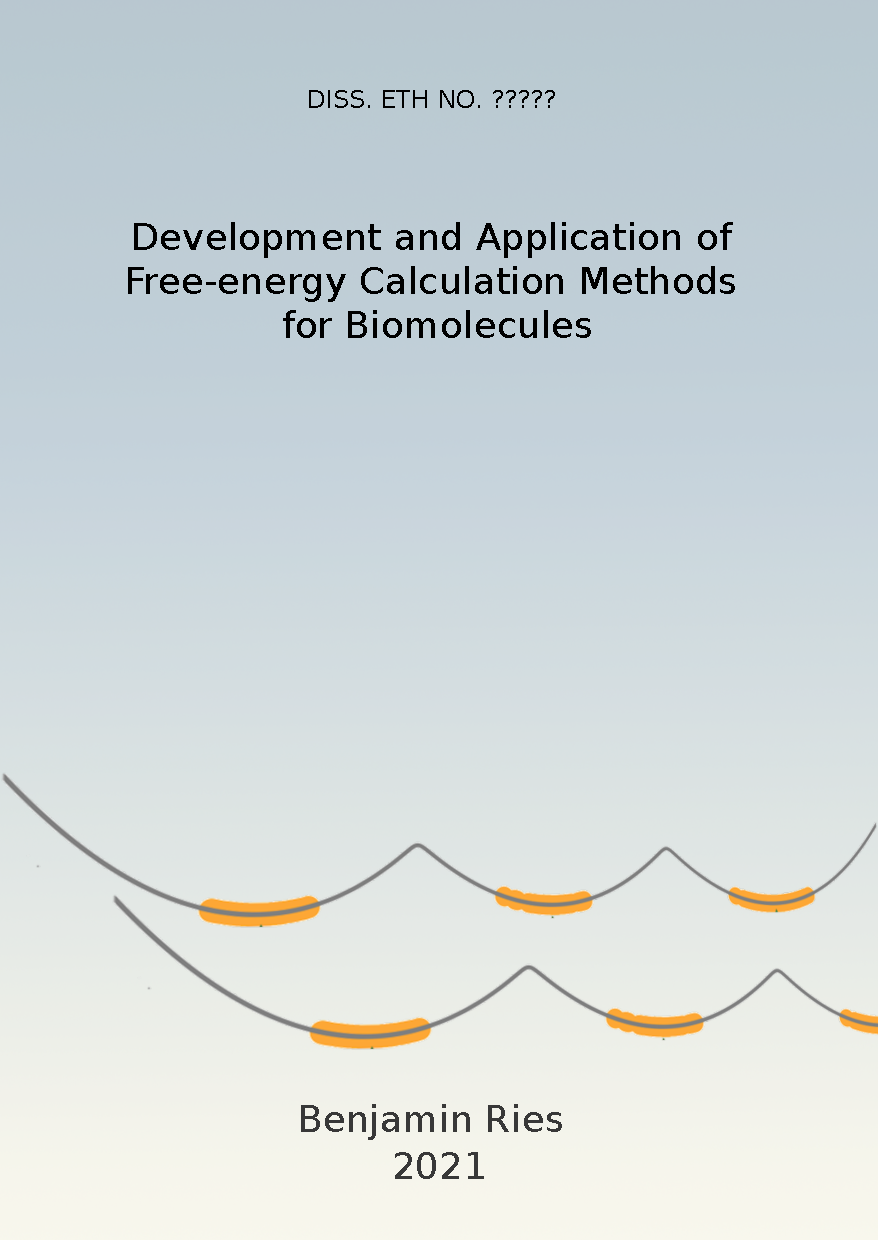
\includepdf[pages=-]{0_cover/frontcover.pdf}
 
 \maketitle
 
 \dedication{Here a nice dedication}

 \chapter{Acknowledgements}

to be added (over the Weekend)


 \tableofcontents

 \chapter{Summary}

Molecular dynamics (MD) simulations offer nowadays a valuable 
tool for studying phenomena in chemistry and biology.
%
The history of models in chemistry, as well as the methodological 
and theoretical background of MD is presented in \refch{intro}.

\refch{resa} deals with the application of explicit-solvent molecular dynamics (MD)
simulations to resorcin[4]arene cavitands, which
can adopt a close/contracted (\vase{})
and an open/expanded (\kite{}) conformation.
%
The \vase-\kite{} equilibria of a quinoxaline- and a dinitrobenzene-based 
resorcin[4]arene are investigated in three solvent environments (vacuum, chloroform and toluene)
and at three temperatures (198.15, 248.15 and 298.15 K).
%
The challenge of sampling the millisecond-timescale \vase-\kite{} transition
%, which occurs experimentally
%on the milisecond timescale, represents a challenge in terms of sampling.
%
%It 
is addressed by calculating relative free energies using ball-and-stick local 
elevation umbrella sampling (B\&S-LEUS) to promote interconversion transitions.
%
The calculated \vase-to-\kite{} free-energy changes $\Delta G$
% between \vase{} and \kite{} calculated
are in qualitative agreement with the 
experimental magnitudes and trends.
%


\refchs{cbti}-\refchnn{cbus} present the development of the conveyor belt scheme,
a method to calculate free-energy differences.
%
The working principle relies on $K$ coupled replicas of the system that are 
simulated at different values of a coupling parameter $\lambda$.
%
The number $K$ is taken to be even and the replicas are equally spaced
on a forward-turn-backward-turn path, akin to a conveyor belt (CB)
between the two end-states.
%
As in $\lambda$-dynamics ($\lam$D), the $\lambda$-values associated with the 
individual systems evolve in time along the simulation.
%
However, they do so in a concerted fashion, determined by the evolution
of a single dynamical variable $\Lambda$ of period $2\pi$ controlling 
the advance of the entire CB.
%
Thus, a change of $\Lambda$ is always
associated with one half of the replicas moving forward and the other half moving backward along $\lambda$.
%
As a result, the effective free-energy profile of the 
replica system along $\Lambda$ is characterized with 
decrasing barriers upon increasing $K$, at least as $K^{-1}$ \radd{in the limit of large $K$}.
%
When \radd{a sufficient number of replicas is used}, 
these variations become small, 
which enables a complete and quasi-homogeneous coverage of the $\lambda$-range
by the replica system.
%


\refch{cbti} introduces this scheme with respect to
alchemical free-energy calculations. Therefore it is termed \textit{conveyor belt thermodynamic integration}.
It provides the mathematical/physical formulation of the scheme, along with an initial 
application of the method to the calculation of the hydration free energy of methanol.

In \refch{ortho}, the conveyor belt thermodynamic integration is applied to 
a Lys-X-Lys tripeptide, involving a side-chain mutation in the central residue,
and guanosine triphosphate, involving a hydrogen-to-bromine mutation.
With both systems, sampling issues have been encountered, due to 
the large orthogonal barriers either along the backbone 
dihedral angles $\phi$ and $\psi$ (tripeptide) or along 
ribose-base dihedral angle $\chi$ (guanosine). 
This relative merits of different sampling schemes, orthogonal biasing and estimators to improve the convergence 
are investigated.
%
%
The thermodynamic integration scheme is shown to suffer from the 
constraint of simulations at fixed $\lambda$.
%
There is no significant improvement upon changing 
from the Simpson's quadrature to the MBAR estimator.
%
Both Hamiltonian replica exchange and conveyor belt 
thermodynamic integration improve the results for
the tripeptide.
%
For the guanosine triphosphate, improvement
is only achieved upon application of an orthogonal biasing potential, 
most efficiently in combination with Hamiltonian replica exchange or
conveyor belt thermodynamic integration.
%

The conveyor belt scheme is extended to the calculation of
conformational free-energy differences in \refch{cbus},
resulting in a so-called conveyor belt umbrella sampling scheme (\CBUS).
%
CBUS is here initally applied to the calculation of 45 standard absolute binding free energies 
of five alkali cations to three crown ethers in three different solvents.
%
Besides introducing and testing the new scheme, it is compared to 
other methods.
%
Expectedly, the direct counting approach has convergence issues
on the accessible simulation timescale, and the corresponding results
are rather unreliable. On the other hand, the results obtained 
using traditional umbrella sampling and CBUS are
very consistent. 
%
Additionally, comparison of the results to
those of previous alchemical calculations {\em via} an
alchemical pathway reveals excellent 
consistency while the trends of available experimental data
are qualitatively reproduced.

Conclusions and an outlook into future developments
are given in \refch{outlook}.

 \chapter{Zusammenfassung}
Die computergestützte Berechnung von Freie Energiedifferenzen ist ein grundlegender Bestandteil der \textit{in silico} Wirkstoffentwicklung. Rigorose Methoden zur Freie Energieberechnung basieren auf Molekulardynamik-Computersimulationen (MD-Simulationen). Kapitel \ref{ch:intro} beinhaltet eine Zusammenfassung der grundlegenden Konzepte von MD-Simulationen. 
Die darauf folgenden Kapitel \ref{ch:feens} - \ref{ch:fereeds} beschreiben Entwicklungen im Bereich computergestützter Freie Energieberechnung. 
In Kapitel \ref{ch:feens} wird das Softwarepaket Ensembler vorgestellt. Dieses kann verwendet werden, um schnell einfache Modelle für die Methodenentwicklung oder für Lehrzwecke zu generieren. In einem eindimensionalen Modellansatz werden verschiedene computergestützte Freie Energieberechnungsmethoden verwendet und miteinander verglichen. 
Kapitel \ref{ch:feres} beinhaltet eine Einordnung für Systemrepräsentationen in relativen Freie Energieberechnungsmethoden. Zudem wird ein Algorithmus vorgestellt, der mehrere Moleküle mittels (lokal) optimaler Distanzdefinitionen für verknüpfte duale Topologien verbindet. Der entwickelte Algorithmus kann mit komplexen Ligandtransformationen, wie sie bei ``Scaffold hopping'' vorkommen, umgehen. Die Mächtigkeit des Algorithmus' wird am Beispiel der Berechnung von Hydratisierungsenergie-Differenzen aufgezeigt.
In Kapitel \ref{ch:fereeds} werden Fortschritte in der RE-EDS Methodik präsentiert, welche auf Modifizierungen im automatischen Optimierungsprozess beruhen. Diese Modifizierungen stellen in erster Linie eine ausreichende Repräsentation jedes Endzustandes in der Simulation sicher. Die verbesserte Pipeline wird auf ein komplexes Liganden-Protein System angewandt, um das Potential der Methode aufzuzeigen.

In Kapitel \ref{ch:pyGrom} wird die Python-Programmierschnittstelle (API) PyGromosTools vorgestellt. Die API ermöglicht den Zugriff auf GROMOS-Dateien, die Generierung von GROMOS-Systemen, die Durchführung von Simulationen sowie die Analyse der generierten Daten. Die Funktionalität der API wird anhand mehrerer Anwendungsbeispiele verdeutlicht.
Kapitel \ref{ch:cycPep} untersucht das konformationelle Verhalten von Paaren von semipeptidischen Makrozyklen, die sich in einem chiralen Zentrum unterschreiben, und verknüpft dieses mit der gemessenen passiven Membranpermeabilität. Die Änderung des chiralen Zentrums führte in einem Makrozyklenpaar zu einer starken  Ver{\"a}nderung der Membrangängigkeit. Die Resultate der Computersimulationen werden mittels NMR-Messungen experimentell validiert.
Das letzte Kapitel rekapituliert die Dissertation und gibt einen Ausblick auf  mögliche Weiterentwicklung der Dissertationsthemen.



 \chapter{Publications}

The following publications are included in parts or in an extended version in this
thesis. The other chapters are in preparation for publication.

\subsection*{Chapter 1}

B.\ Ries, S.\ M.\ Linker, D.\ F.\ Hahn, G.\ K\"onig, S.\ Riniker {\em J. Chem. Inf. Model.} {\bf 2021}: 
Ensembler: A Simple Package for Fast Prototyping and Teaching Molecular Simulations


\subsection*{Chapter 2}

B.\ Ries, K.\ Normak, R. G.\ Wei\ss, S.\ Rieder, C.\ Candide, G. K\"onig, S.\ Riniker {\em J. Comput. Aided Mol. Des.} {\bf 2021}, {\em submitted}: 
Relative Free-Energy Calculations for Scaffold Hopping-Type Transformations with an Automated RE-EDS Sampling Procedure



 \mainmatter
\subfile{2_chapter_intro/content_introduction.tex}
\subfile{3_chapter_1/content_chapter1.tex}
\subfile{4_chapter_2/content_chapter2.tex}
\subfile{5_chapter_3/content_chapter3.tex}
\subfile{6_chapter_4/content_chapter4.tex}
\subfile{7_chapter_5/content_chapter5.tex}
\chapter{Outlook}
\label{ch:outlook}

\aquote{
`` tata ''
}
{tutu }



\section{Path Free Multistate Methods for RE-EDS}


\section{Software Development in Computational Chemistry and Gromos}


\section{Cyclic Peptides}


%

 
 \backmatter
  \addcontentsline{toc}{chapter}{References}
  \bibliography{
  	2_chapter_intro/ref/ref.bib,
  	3_chapter_1/ref/ref.bib, 
  	4_chapter_2/ref/ref.bib,
  	5_chapter_3/ref/ref.bib,
  	6_chapter_4/ref/ref.bib,
  	7_chapter_5/ref/ref.bib
	}

 %%%%%%%%%%%%%%%%%%%%%%%%%%%%%%%%%%%%%%%%%%%%%%%%%%%%%%%%%%%%%%%%%%%%
\chapter{Curriculum Vit\ae}
\definecolor{awesome-skyblue}{HTML}{0395DE}
\colorlet{awesome}{awesome-skyblue}
\vspace{-1cm}
\cvsection{Benjamin Joachim Ries}
\begin{cvlist}
\cventry{15.03.1991}{}
\cventry{Ettlingen, Germany}{}
\cventry{German citizen}{}
\end{cvlist}

\cvsection{Education}
\begin{cvlist}
\cventry
    {PhD, ETH Z\"{u}rich } % Degree
    {2017 -- 2021} % Date(s)
\cventry
    {Bioinformatics MSc., Universit\"{a}t T\"{u}bingen} % Degree
    {2012 -- 2014} % Date(s)
\cventry
    {Biochemistry BSc., Universit\"{a}t T\"{u}bingen} % Degree
    {2009 -- 2013} % Date(s)
\cventry
    {secondary school examinations (Abitur), Albertus Magnus Gymnasium, Ettlingen, Germany} % Location
    {2002 -- 2011} 
\end{cvlist}
\vspace{-0.5cm}
\cvsection{Experience}
\begin{cvlist}
	\cventry
	{Summerschool,  Universita della Svizzera Italiana, Switzerland: Effective High-Performance Computing \& Data Analytics with GPUs} % Degree
	{2019} % Date(s)
	\cventry
	{Summerschool,  University of Jyväskylä, Finland: Measuring and Modelling Proton Equilibria in Complex Macromolecular Systems} % Degree
	{2017} % Date(s)
	
	\cventry
	{Erasmus+ internship, Uppsala Universitet, Sweden} % Degree
	{2016 -- 2017} % Date(s)
	
	\cventry
    {Lab Assistant, MPI, Developmental Biology, T\"{u}bingen} % Institution
    {2013 -- 2014} % Date(s)
\end{cvlist}
\vspace{-0.75cm}
\cvsection{Teaching Assistant}
\begin{cvlist}
	\cventry
	{Physical Chemistry I: Thermodynamics (spring semester), F.\ Merkt} % Degree
	{2018} % Date(s)
	\cventry
	{Algorithms and Programming in C++ (autumn semester), S.\ Riniker} % Degree
	{2018, 2019} % Date(s)
	\cventry
	{Physical Chemistry Practicum for Biology and Pharmacy Students: Molecular Dynamics (spring semester), E.\ Meister} % Degree
	{2019, 2020} % Date(s)
	\cventry
	{Statistical Physics and Computer Simulation for CSE (spring semester), P.\ H\"unenberger and S.\ Riniker} % Degree
	{2021} % Date(s)
\end{cvlist}
\vspace{-0.75cm}
\cvsection{Commitment}
\begin{cvlist}
	\cventry
	{young swiss chemical society (youngSCS), ETH Representative (2019-2020), President(2020-2021)} % Degree
	{2019-2021} % Date(s)
	\cventry
	{juniorGBM T\"ubingen, president(2016)} % Degree
	{2012-2017} % Date(s)
	
\end{cvlist}


\end{document}

